\newpage
\section{Introduction}
\label{Introduction}

The observations conducted in the lab session centered around observing thermodynamic processes inside a metal cylinder, verifying its properties as an ideal gas and determining work and heat involved when undergoing an Ericsson cycle. Furthermore, the engine's efficiency will be compared to that of the Carnot cycle.  

The explicit notion of viewing heat and work as two closely related energy quantities is rather novel compared to the long history in which the practical implications were already utilized. The first steam engine, although severely lacking in its efficiency, had already been implemented in Britain as early as 1698, and optimized by Newcomen and Watt in the subsequent century \cite{Saslow2020AHO}. Later, the rate of development sped up during the peak of the industrial revolution, where efforts were aimed at improving the efficiency of existing engines \cite{LumenLearning}. In 1824, Sadi Carnot proposed in 1824 the Carnot Cycle as a reversible heat engine, consisting of two isothermal and two adiabatic processes, while also introducing the idea of separate hot and cold reservoirs in which the engines would operate. \cite{Saslow2020AHO}

These achievements were based on a complex history of discoveries, and continued to be. Independently, several scientists reached the conclusion that the internal energy of an isolated system has to stay constant, but can vary in its form, later regarded as the First Law of Thermodynamics. Entropy, its property as a state function and its change under reversible and irreversible processes were outlined in 1865 by Rudolf Claudius \cite{Saslow2020AHO}. These concepts and numerous others lay the foundations of thermodynamics, which can be classified as the study of macroscopic properties of a system, as a result of its molecular behaviour. \cite{LabManual}

\subsection{Theory}
\label{Theory}

The experimental setup includes a metal can which is later connected to a piston tube expanding under higher pressure. By preparing separate heat reservoirs, one can simulate a cycle which the gas undergoes. More precisely, if the gas can be thought of as an ideal gas, the cycle will consist of two isobaric and two adiabatic processes. In between, heat is converted into mechanical work, and it is therefore fundamental to understand the principles behind ideal gasses and thermodynamic processes.

\subsubsection{Ideal Gas Law}
\label{Ideal Gas Law}

In thermodynamics, the key characteristics of a gas system considered in calculation are the pressure $\mathit{P}$, volume $\mathit{V}$, temperature $\mathit{T}$ and the amount of it. The latter is often represented in the number of moles of gas $\mathit{n}$, which equates to $\mathit{N_A = 6.022 \cdot 10^{23}}$ individual molecules. These can be used to define define properties such as internal energy $\mathit{E_{int}}$ or work $\mathit{W}$ for specific situations. By holding certain parameters constant, a number of underlying laws for ideal gasses have been discovered. The assumption of ideal gasses implied an assembly of non-interacting, similar point-like particles performing elastic collisions. Macroscopically, this is a decent approximation for most real processes \cite[pp.~391-395]{Brown}. 

\textbf{Boyle's Law} states that under constant $\mathit{n}$ and $\mathit{T}$, the system's volume is inversely proportional to the pressure: 

\begin{equation}
\label{eq:Boyle's Law}
    \mathit{V \alpha \frac{1}{P}}
\end{equation}

Stated in \textbf{Charles' law}, at constant $\mathit{n}$ and $\mathit{P}$, volume is proportional to the temperature: 

\begin{equation}
\label{eq:Charles' Law}
    \mathit{V \alpha T}
\end{equation}

Note that the absolute temperature scale is is generally applied in thermodynamics, with $\mathit{T}$ measured in Kelvin [K]. Similarly, \textbf{Gay-Lussac's law} related pressure to temperature, under the condition that $\mathit{n}$ and $\mathit{V}$ are held constant. It can already be implied from the previous laws: \cite[pp.~387-391]{Brown}

\begin{equation}
\label{eq:Gay-Lussac's Law}
    \mathit{P \alpha T}
\end{equation}

Lastly, \textbf{Avogadro's law} shows that at constant $\mathit{T}$ and $\mathit{P}$, volume is proportional to the number of moles contained in it: \cite[pp.~387-391]{Brown}

\begin{equation}
\label{eq:Avogadro's Law}
    \mathit{V \alpha n} 
\end{equation}

% https://chem.libretexts.org/Bookshelves/General_Chemistry/Map%3A_Chemistry_-_The_Central_Science_(Brown_et_al.)/10%3A_Gases/10.03%3A_The_Gas_Laws


Combining the relations and introducing a new constant factor $\mathit{R} = 8.314 \frac{J}{Kmol}$, the gas constant, the \textbf{ideal gas law} appears as a result, as seen in Equation \ref{eq:Ideal_Gas_Law}. As the name suggests, the relation holds true for ideal gases. \cite[pp.~391-395]{Brown}

\begin{equation}
\label{eq:Ideal_Gas_Law}
    \mathit{PV = nRT}
\end{equation}

At higher pressures and temperatures, a bigger deviation from ideality occurs for the gas. Hence, a compressibility factor $\mathit{z}$ is introduced in modern analysis. \cite{AHMED201029}

\subsubsection{Work and Heat}
\label{Work-Heat}

Work is done by application of a force $\mathit{F}$ over a distance $\mathit{dx}$. A gas contained in a tube pushing against a piston would exert a force relative to the pressure and the piston's area. If that force causes a change in volume $\mathit{dV}$, the work applied or exerted on the gas is given by: \cite{Ling2016-bs}

\begin{equation}
\label{eq:Work}
    \mathit{dW = PdV}
\end{equation}

For processes between conditions 1 and 2, one can further modify the equation:

\begin{equation}
\label{eq:Work_Int}
    \mathit{W = \int_{V_1}^{V_2} PdV}
\end{equation}

Work is a path-dependent function, the way chosen to get from A to B has an impact on the resultant work. 

\begin{wrapfigure}{r}{0.4\textwidth}  % 'r' for right, and width of 0.4 of the text width
    \centering
    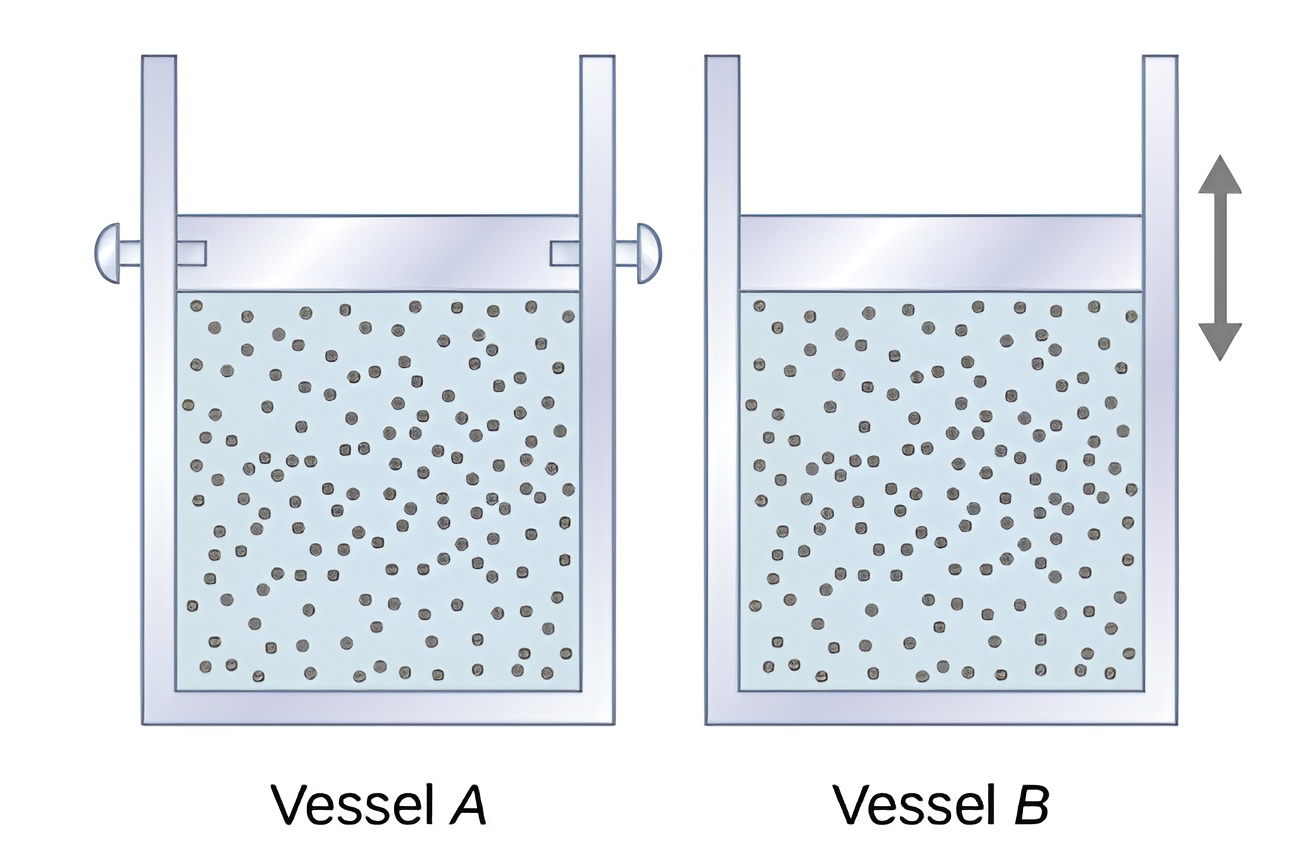
\includegraphics[width=0.4\textwidth]{Graphics/Constant_Diagrams.png}  % Adjust the width of the image
    \caption{Same thermodynamic system, with particles trapped inside a cylinder with a movable piston. Left: Volume is fixed. Right: Pressure is fixed. \cite{Ling2016-bs}  }
    \label{fig:Constants}
\end{wrapfigure}

The other relevant type of energy exchange can be classified as that of heat $\mathit{Q}$. Heat describes the transfer of energy into or out of the system, where $\mathit{Q}$ is negative or positive depending on the convention in which direction heat flow is described \cite{Ling2016-bs}. The amount of heat that is expelled is based on the change in temperature of the system, but also dependent on the number of atoms per molecule, which decides the degrees of freedom of movement. The relationship can be summarized in Equation \ref{eq:Heat}. \cite{Zohuri2019}

\begin{equation}
\label{eq:Heat}
    \mathit{Q = mc \Delta T}
\end{equation}

where $\mathit{m}$ represents mass and $\mathit{c}$ is the heat specific heat. 

The equation can be simplified under specific constraints, which is visualized in Figure \ref{fig:Constants}. If one would fix the piston such that the volume stays the same, the heat related to an infinitesimally small temperature change is given by Equation \ref{eq:C_V}. \cite{Zohuri2019}

\begin{equation}
\label{eq:C_V}
    \mathit{dQ = n C_V dT}
\end{equation}

At constant pressure, Equation \ref{eq:Heat} becomes. 

\begin{equation}
\label{eq:C_P}
    \mathit{dQ = n C_P dT}
\end{equation}

A thermodynamic system contains an internal energy $\mathit{U}$. The total heat exchanged and work done by the system are related in the First Law of Thermodynamics: 

\begin{equation}
\label{eq:1st Law}
    \mathit{\Delta U = Q - W}
\end{equation}

For any process between two equilibrium states, the law should be applicable. \cite{Ling2016-bs}


\subsubsection{Heat Engines and Thermodynamic Processes}
\label{Heat Engines}

\begin{wrapfigure}{r}{0.35\textwidth}  % 'r' for right, and width of 0.4 of the text width
    \centering
    \vspace{-0.75cm}
    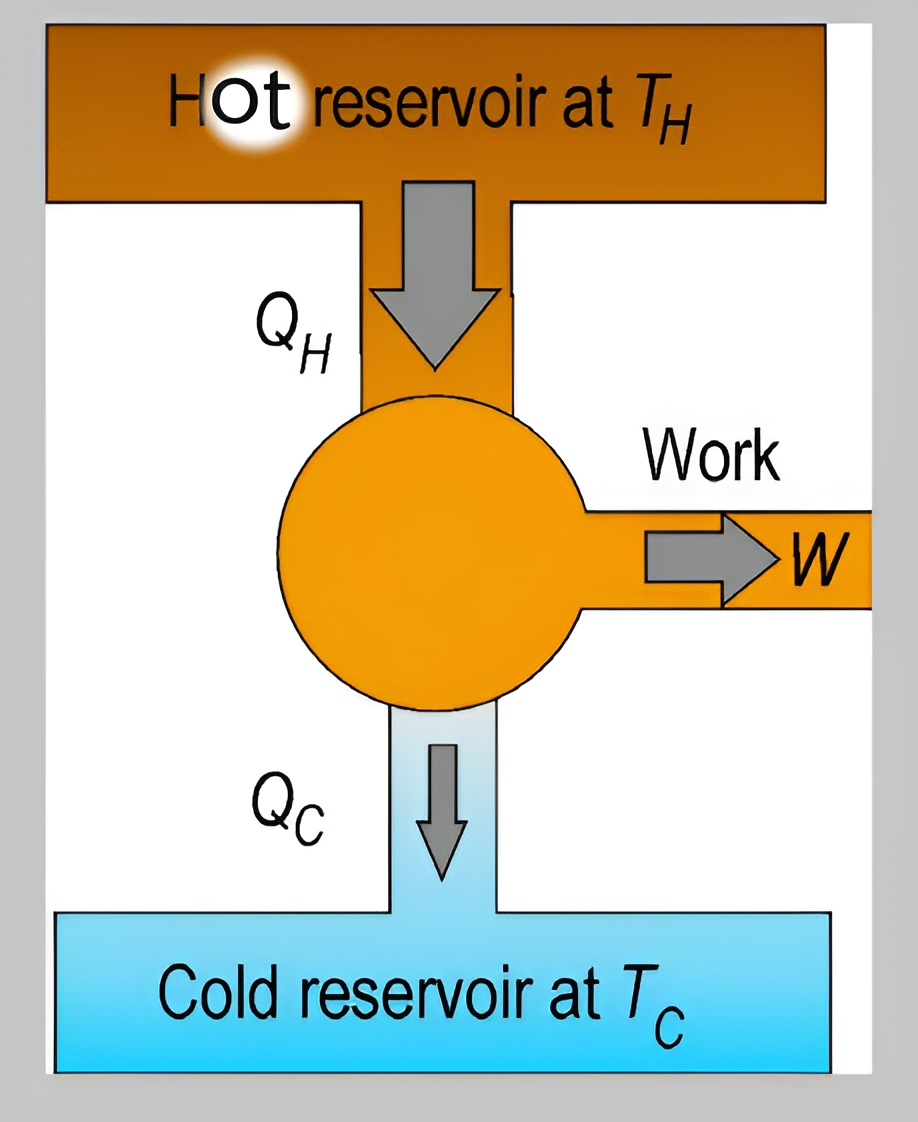
\includegraphics[width=0.35\textwidth]{Graphics/Heat_Engine.png}  % Adjust the width of the image
    \caption{PV-Diagram of the Carnot Cycle. \cite{Bassie2012-pw}}
    \label{fig:Carnot Cycle}
\end{wrapfigure}

In thermodynamics, one usually refers to a system as the part of the universe for which the observations are taken. One is especially interested in the changes in states when interactions with the environment occur. If non-quasi-static, only the beginning and ending state during these thermodynamic processes can be described at thermal equilibrium. In theory, one could slow down the transition to a point where the system appear to always be in thermal equilibrium. \cite{Ling2016-bs}

Heat engines are designed to extract heat and, by cycling through specific types of thermodynamic processes, translate it into work and arrive at the same thermal equilibrium state. The efficiency of each cycle for a given machine is defined by Equation \ref{eq:Efficiency}.

\begin{equation}
\label{eq:Efficiency}
    \mathit{\nu = \frac{W}{Q_h} = 1 - \frac{Q_c}{Q_h}}
\end{equation}

Key to the cyclic nature is a setup consisting of one high-temperature and one cold-temperature reservoir. In the equation, $\mathit{Q_h}$ represents the heat withdrawn from the hot reservoir, $\mathit{W}$ the work delivered and $\mathit{Q_c}$ the heat disposed in the cold reservoir during each cycle. 

The Carnot Cycle is the ideal model for a heat engine. Consisting of two adiabatic and two isothermal processes, it is the cycle with the maximum possible efficiency. The steps are visualized in Figure \ref{fig:Carnot Cycle}, where the area enclosed by the graphs is the net work of the heat engine.

\begin{figure}[H] % 'r' for right, and width of 0.4 of the text width
    \centering
    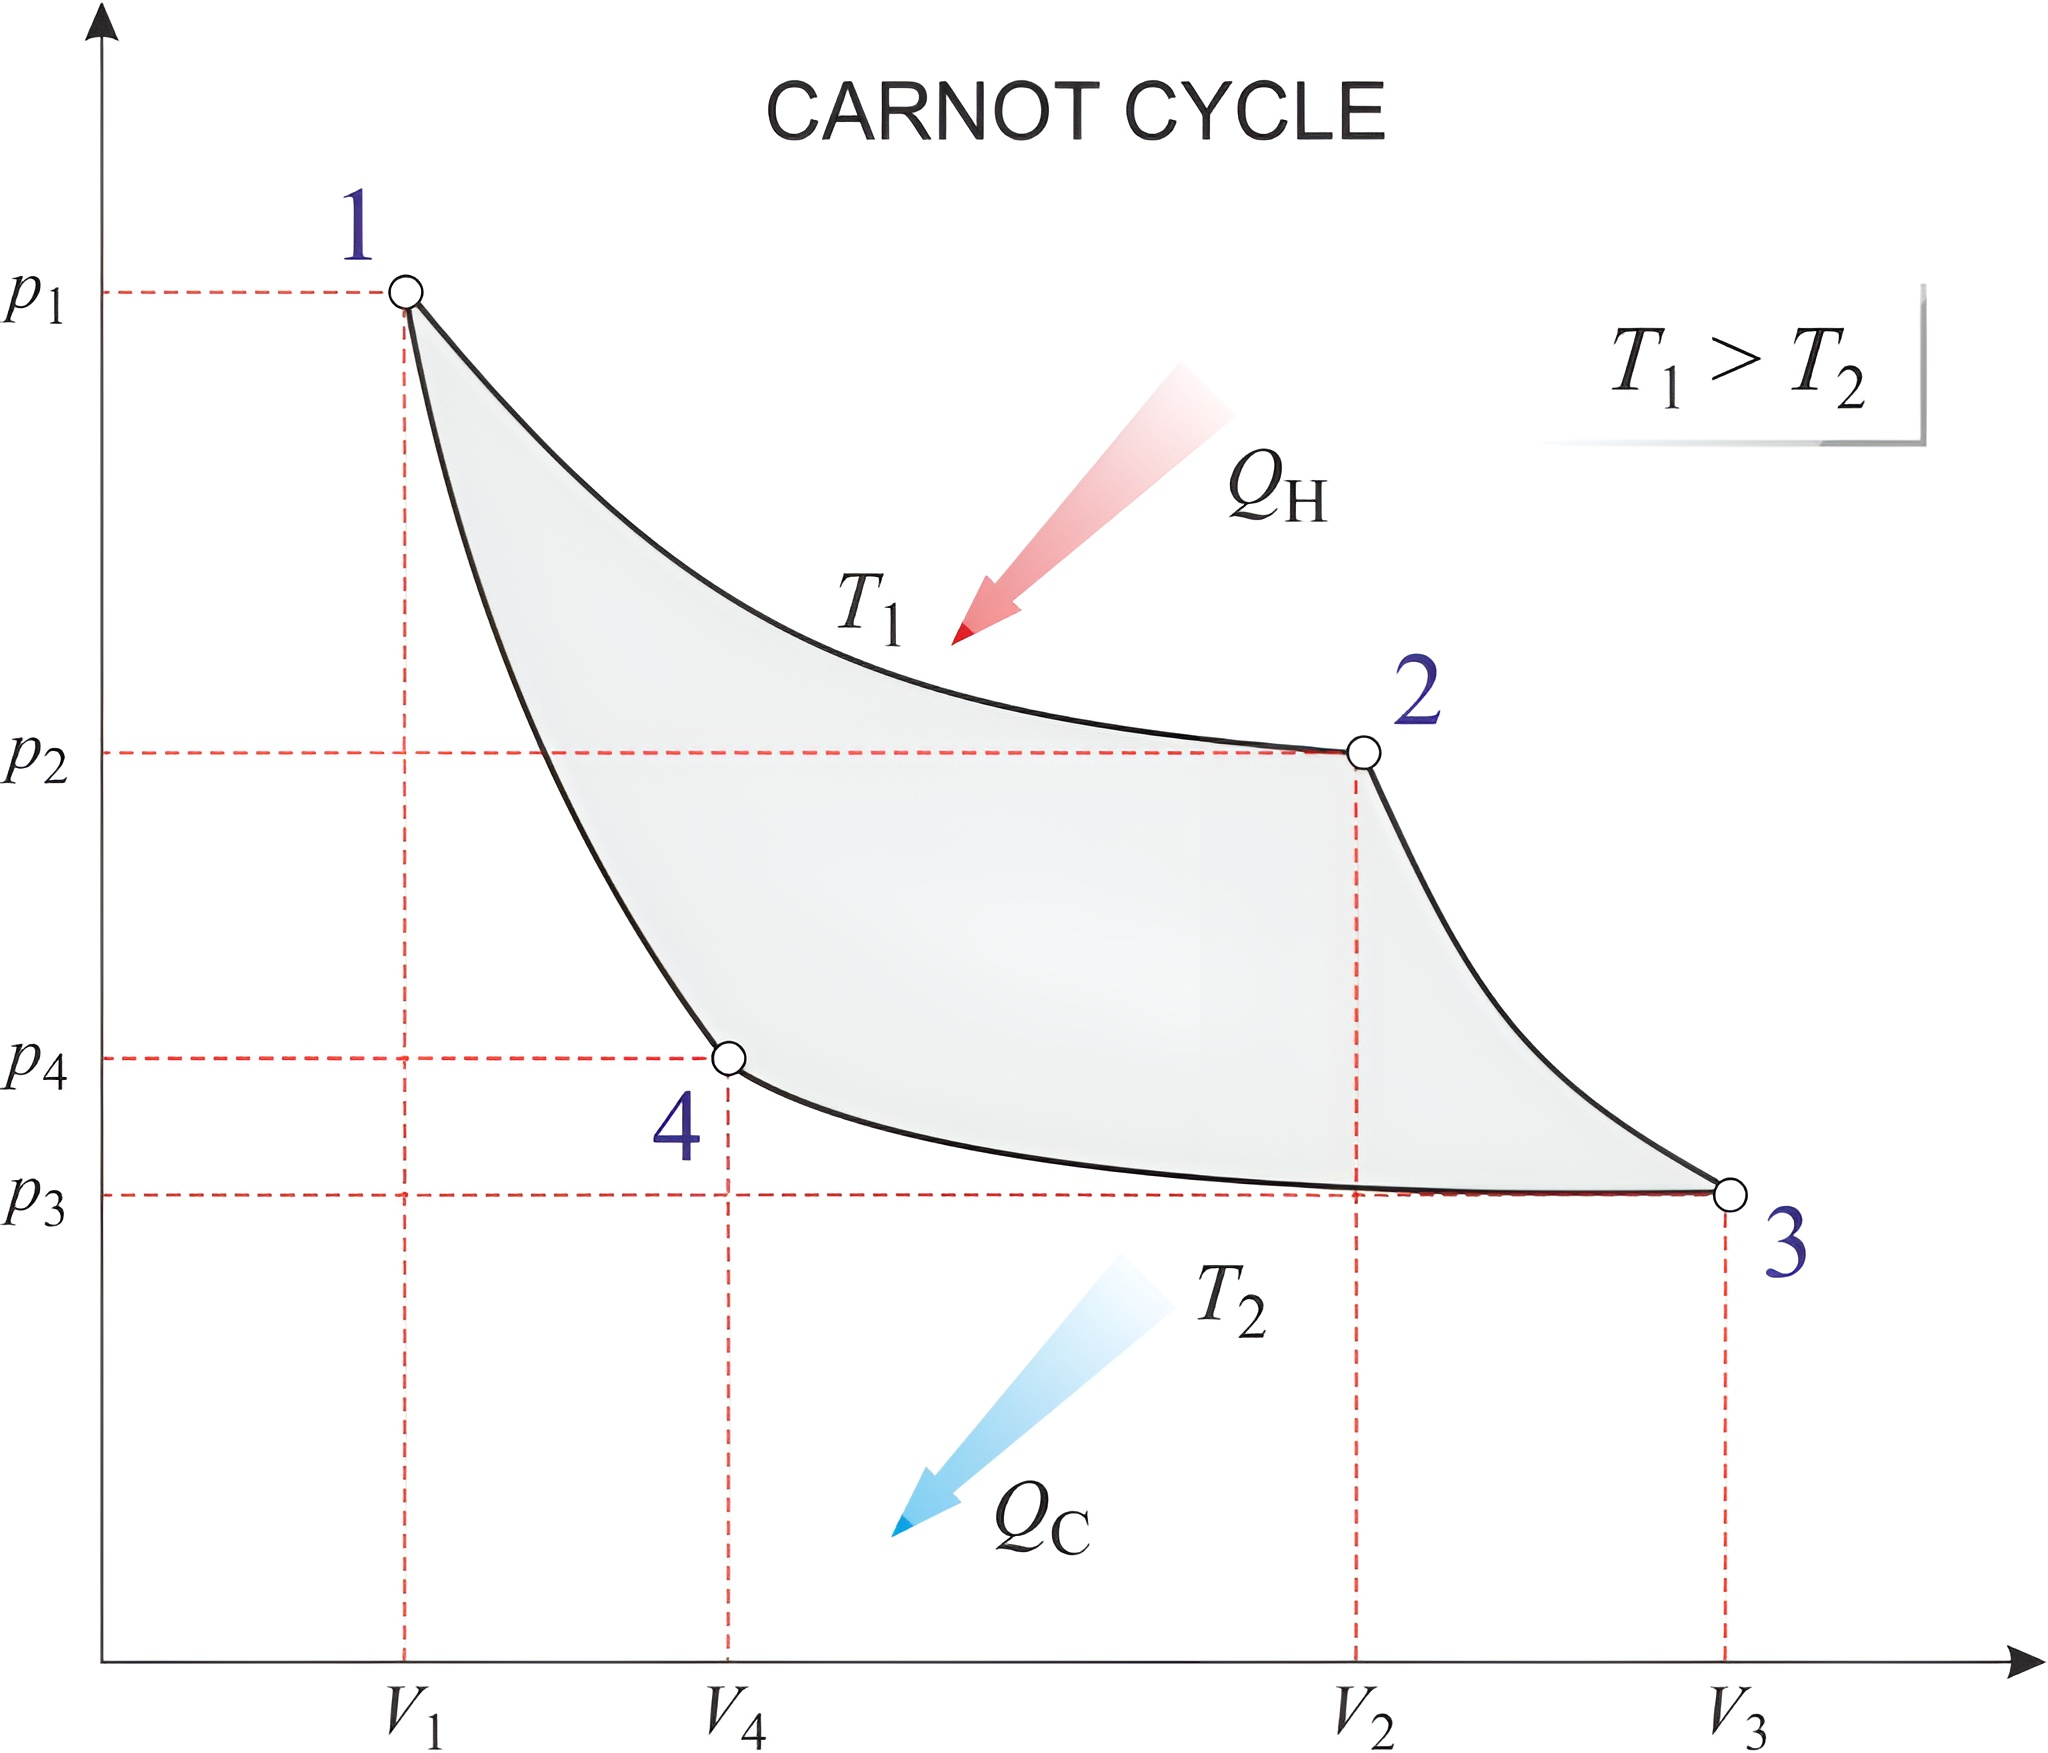
\includegraphics[width=0.4\textwidth]{Graphics/Carnot_Cycle.png}  % Adjust the width of the image
    \caption{PV-Diagram of Carnot Cycle: Heat is extracted from the hot reservoir, some of it is converted into work and some passed onto the cold reservoir. \cite{Eni}}
    \label{fig:Carnot_Cycle}
\end{figure}

Note that any of the steps outlined below can be the starting point: \cite{DINCER2018125}


% refer to figure
\begin{enumerate}
    \item \textbf{Isothermal expansion (1-2)}: Heat is absorbed from the hot reservoir at constant temperature, until equilibrium is reach. In the process, the volume grows.
    \item \textbf{Adiabatic compression (2-3)}: Gas stays in the same reservoir without heat transfer. Permitting it to expand the volume, the gas will deliver work in an adiabatic expansion.
    \item \textbf{Isothermal compression (3-4)}: Heat is transferred to the cold reservoir at constant temperature, until equilibrium is reached. The volume shrinks as a result.
    \item \textbf{Adiabatic expansion (4-1)}: Gas stays in the same reservoir without heat transfer. Work is done on the gas, transforming the gas into its original thermodynamic state. 
\end{enumerate}

For an ideal gas Carnot Cycle, the efficiency is simplified: \cite{BARBIR201317}

\begin{equation}
\label{eq:Carnot_Efficiency}
    \mathit{\eta = 1 - \frac{T_c}{T_h}}
\end{equation}

Using the same hot and cold reservoirs, work can be produced over a variety of processes. That being said, the efficiency of any other cycle has to be lower than the one calculated in Equation \ref{eq:Carnot_Efficiency}.

\subsection{Hypothesis}
\label{Hypothesis}

The first part of the lab session centers around verifying that the gas contained in the tube can be considered ideal. Although air is composed of multiple types of molecules, the majority of them could be considered to act similarly. Air can definitely not be considered an ideal gas, especially due to interactions between the molecules, but its macroscopic behaviour under the temperature and pressure conditions involved should somewhat match that exhibited by an ideal gas.

In the second part, the apparatus will be tested on a specific cycle. Using these results, one can calculate the heat engine's efficiency and compare it to the one theoretically obtained by a Carnot cycle. The heat engine's efficiency is expected to be far lower than the Carnot efficiency, mainly due to the simplicity of the setup. Additionally, leaks and frictional forces could affect the results, leading to higher deviations.